\subsection{Miglioramento dei processi}
Il Gruppo \Gruppo{} ha deciso di adottare il ciclo di Deming. Il ciclo di Deming è un metodo di gestione iterativo per il controllo e il miglioramento continuo dei processi (e anche dei prodotti) suddiviso in 4 fasi: Plan, Do, Check e Act. 
Anche la norma ISO/IEC 12207 utilizza questo ciclo per scopi di miglioria dei \glo{processi}. Per garantire la qualità dei \glo{processi} e la coerenza allo standard, il gruppo \Gruppo{}  
ha scelto di adottare il ciclo PDCA.

\begin{figure}[h]
    \centering
    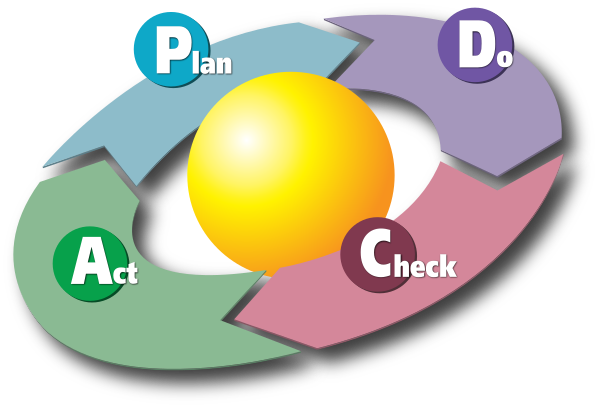
\includegraphics[scale=0.2]{Sezioni/Immagini/PDCA.png}
    \caption{Ciclo PDCA - Plan Do Check Act}
\end{figure}

\textbf{Fasi del ciclo PDCA:}
\begin{itemize}
    \item \textbf{Plan}: Definisce attività e scadenze necessarie al raggiungimento dei specifici obiettivi di miglioramento;
    \item \textbf{Do}: Esegue le attività di "Plan";
    \item \textbf{Check}: Verifica l'esito delle azioni di miglioramento rispetto alle attese. Si analizzano i risultati del "Do" e li si confrontano con gli obiettivi individuati nel "Plan";
    \item \textbf{Act}: Consolida il tutto e cerca dei metodi per il prossimo miglioramento. Se il "Check" ha dimostrato che il "Plan" implementato dal "Do" è migliore rispetto ai precedenti \glo{processi} standard, allora questo piano diventa il nuovo \glo{processo} standard. Altrimenti il vecchio standard in uso rimarrà la \glo{baseline}.
\end{itemize}